\documentclass[12pt]{article}
\usepackage{fullpage}
\usepackage{titlesec}
\usepackage{tikz}
\usepackage{amsfonts,amssymb}
\usepackage{amsmath}
\usepackage{comment}
\usetikzlibrary{automata, positioning}

\pagestyle{plain}
\titleformat{\subsection}[runin]
  {\normalfont\large\bfseries}{\thesubsection}{1em}{}

\title{Homework 2}
\author{Brooke Fugate, Michael O'Connor, Rohan Shah}
\date{}

\begin{document}
\maketitle

\section*{Problem B1}

\subsection*{(a)}
NFA with $2n+1$ states accepting $L_n$:
\newline
\begin{center}
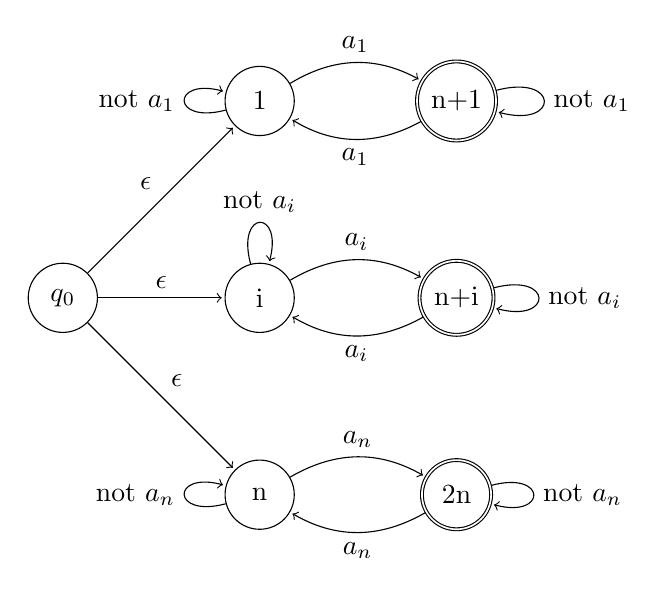
\begin{tikzpicture}[shorten >=1pt, node distance=2.5cm, on grid, auto]
  \node[state] (q0) {$q_0$};
  \node[state] (q2) [right=of q0] {i};
  \node[state] (q1) [above=of q2] {1};
  \node[state] (q3) [below=of q2] {n};
  \node[state, accepting] (q4) [right=of q1] {n+1};
  \node[state, accepting] (q5) [right=of q2] {n+i};
  \node[state, accepting] (q6) [right=of q3] {2n};
  \path[->]
  (q0) edge node {$\epsilon$} (q1)
       edge node {$\epsilon$} (q2)
       edge node {$\epsilon$} (q3)
  (q1) edge [loop left] node {not $a_1$} (q1)
  (q1) edge [bend left] node {$a_1$} (q4)
  (q4) edge [loop right] node {not $a_1$} (q4)
  (q4) edge [bend left] node {$a_1$} (q1)
  (q2) edge [loop above] node {not $a_i$} (q2)
  (q2) edge [bend left] node {$a_i$} (q5)
  (q5) edge [loop right] node {not $a_i$} (q5)
  (q5) edge [bend left] node {$a_i$} (q2)
  (q3) edge [loop left] node {not $a_n$} (q3)
  (q3) edge [bend left] node {$a_n$} (q6)
  (q6) edge [loop right] node {not $a_n$} (q6)
  (q6) edge [bend left] node {$a_n$} (q3)
  ;
\end{tikzpicture}
\end{center}
\subsection*{(b)}
  We can construct a DFA $D_i$ for each language $L^i_n$, where $L^i_n$ is the
  set of all strings over $\Sigma$ with an odd number of $a_i$, using two states
  as shown below. Since $L_n$ is the union of all such $L^i_n$, i.e.
  $L_n = L^1_n \cup \dots \cup L^n_n$ where $n$ is the number of symbols in the
  alphabet $\Sigma$, we can use the cross-product construction to combine each
  DFA $D_i$ and create a DFA $D$ that accepts the language $L_n$.
  The cross-product construction creates a DFA with $2^n$ states (since there
  are 2 states per DFA $D_i$ and thus the number of states in $D$ is doubled
  with each construction or n times). Thus there exists a DFA $D$ with $2^n$
  states that accepts the language $L_n$.
  \vspace{0.5cm}
  Below is a DFA $D_i$ that accepts the language $L^i_n$ using two states:
  \newline
  \begin{center}
  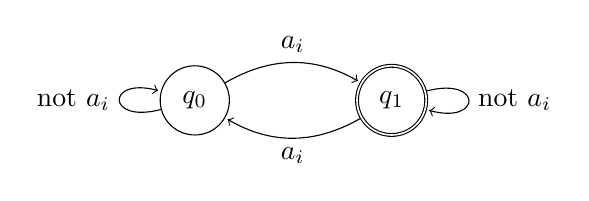
\begin{tikzpicture}[shorten >=1pt, node distance=2.5cm, on grid, auto]
    \node[state] (q0) {$q_0$};
    \node[state, accepting] (q1) [right=of q0] {$q_1$};
    \path[->]
    (q0) edge [bend left] node {$a_i$} (q1)
    (q0) edge [loop left] node {not $a_i$} (q0)
    (q1) edge [bend left] node {$a_i$} (q0)
    (q1) edge [loop right] node {not $a_i$} (q1)
    ;
  \end{tikzpicture}
  \end{center}

\subsection*{(c)}
Proof by contradiction:\newline
\indent Assume that that there is a DFA $D_{bad} = (Q, \Sigma, \delta, q_0, F)$ such that $D_{bad}$ has less than $2^n$ states and it accepts the language $L_n$. Since we know that $L_n$ is a regular language from part b we know that there is some Myhill-Nerod relation such that $x \simeq_D y$. This means there is some state $p \in F$ that will accept strings $x, y$ such that $x$ has an even number of $a_i$ and $y$ has an odd number of $a_i$. Then we can construct a string $z$ that will set every other $a_j$ to even: i.e. $x = a_1a_2a_3 , y=a_1a_2a_3a_3 , z=a_1a_2$.  This would mean that $xz \simeq_D yz$ and $xz \in L_n but yz \notin L_n$ which is a contradiction. So a DFA with less than $2^n$ states can not accept $L_n$ and from part b we showed that a DFA with $2^n$ states is accepting of $L_n$ so a DFA accepting $L_n$ must have at least $2^n$ states.

\section*{Problem B2}
\subsection*{(a)}
Let DFA $D_C = (Q, T, \delta_C, q_0, F_C)$ be a DFA that accepts the language: \[
C = \{u\in T^3 \mid u \notin \{110, 111, 112, 101, 121, 011, 211\}\}
\]
\begin{center}
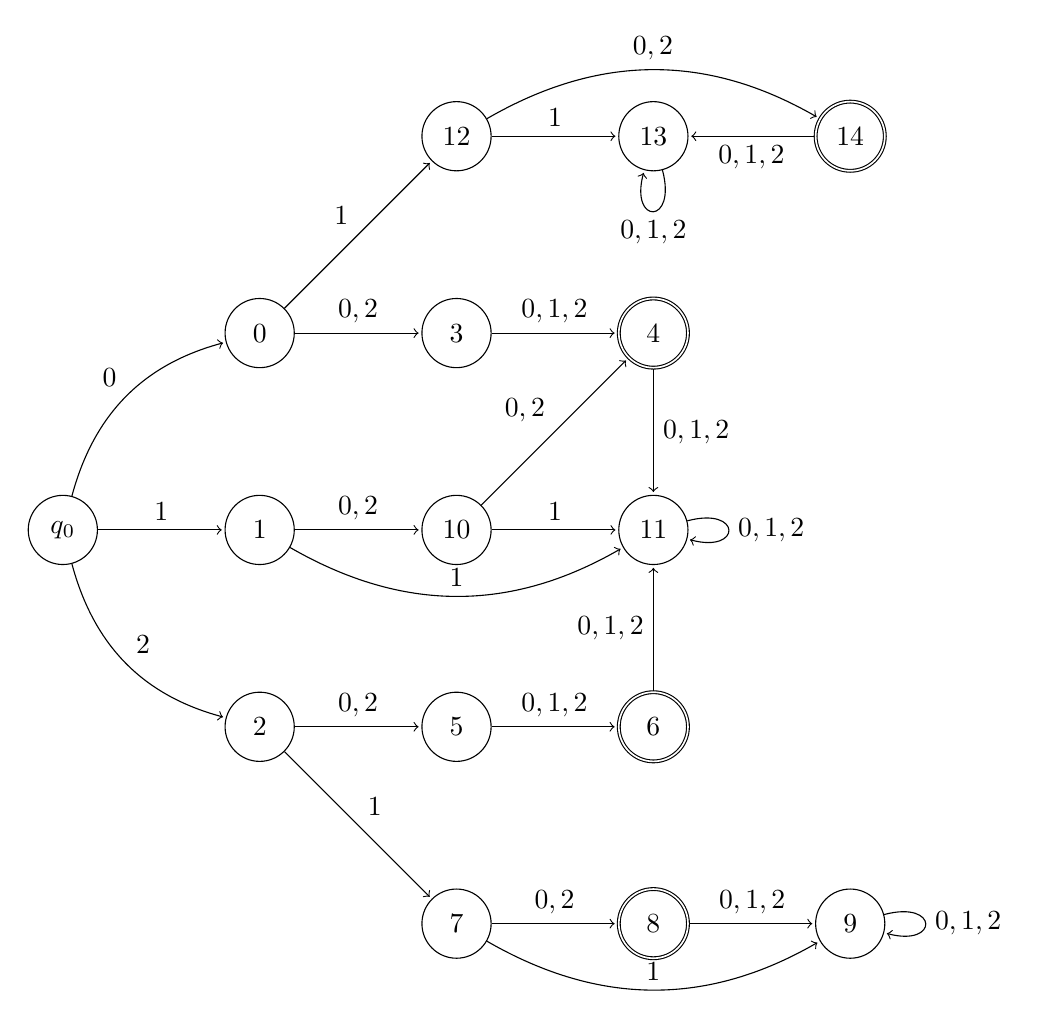
\begin{tikzpicture}[shorten >=1pt, node distance=2.5cm, on grid, auto]
  \node[state] (q0) {$q_0$};
  \node[state] (q2) [right=of q0] {1};
  \node[state] (q1) [above=of q2] {0};
  \node[state] (q3) [below=of q2] {2};
  \node[state] (q4) [right=of q1] {3};
  \node[state, accepting] (q5) [right=of q4] {4};
  \node[state] (q6) [right=of q3] {5};
  \node[state,accepting] (q7) [right=of q6] {6};
  \node[state] (q8) [below=of q6] {7};
  \node[state,accepting] (q9) [right=of q8] {8};
  \node[state] (q10) [right=of q9] {9};
  \node[state] (q11) [right=of q2] {10};
  \node[state] (q12) [right=of q11] {11};
  \node[state] (q13) [above=of q4] {12};
  \node[state] (q14) [right=of q13] {13};
  \node[state, accepting] (q15) [right=of q14] {14};
  \path[->]
(q0) edge [bend left] node {$0$} (q1)
(q0) edge node {$1$} (q2)
(q0) edge [bend right] node {$2$} (q3)
(q1) edge node {$0,2$} (q4)
(q1) edge node {$1$} (q13)
(q13) edge node {$1$} (q14)
(q13) edge [bend left]node {$0,2$} (q15)
(q2) edge node {$0,2$} (q11)
(q3) edge node {$0,2$} (q6)
(q3) edge node {$1$} (q8)
(q4) edge node {$0,1,2$} (q5)
(q6) edge node {$0,1,2$} (q7)
(q8) edge node {$0,2$} (q9)
(q8) edge [bend right] node {$1$} (q10)
(q10) edge [loop right] node {$0,1,2$} (q10)
(q11) edge node {$0,2$} (q5)
(q11) edge node {$1$} (q12)
(q12) edge [loop right] node {$0,1,2$} (q12)
(q2) edge [bend right] node {$1$} (q12)
(q5) edge node {$0,1,2$} (q12)
(q7) edge node {$0,1,2$} (q12)
(q9) edge node {$0,1,2$} (q10)
(q14) edge [loop below] node {$0,1,2$} (q14)
(q15) edge node {$0,1,2$} (q14)
  ;
\end{tikzpicture}
\end{center}
Let there be a DFA  $D_{Lm} = (Q, T \cup \{c\}, \delta_{Lm}, q_0, F_C)$. $\delta_{Lm}$ is the transition function that has all the same transitions as $\delta_C$ with the following additional transitions:
\begin{center}$\delta_{LM}(q, c) = q_0$ if $q \in F$\end{center}
\begin{center}$\delta_{LM}(q, c) = 11 $ if $q \notin F$\end{center}
Informally this adds a transition that from all states $p \in F_C$ if a letter $c$ is encountered it goes back to $q_0$ and on any $p \notin F_C$ if a letter $c$ is encountered it goes to a bad state.\newline\newline
Proof that $D_{Lm}$ accepts the language $L_m$:\newline
\indent$L_m$ is basically $C^+$ with a c transition between each string in the language $C$: i.e. $u_1cu_2cu_3c....u_n$. $D_Lm$ accepts all $u_i$ because it contains the transition function of $\delta_C$ and the final states $F_C$.  So we need to show that it accepts subsequent $cu$ strings.  $D_{Lm}$ on reaching a $p$ in $F_C$ transitions on a $c$ back to $q_0$, which can then accept a string $u_i$ as described above and repeat.  Any bad string in a $u_b$ will be rejected by the transition function taken from $D_C$ and any non $c$ transition from a final state is thrown into a bad state.  Therefore $D_{Lm}$ accepts the language $L_m$. 
\subsection*{(b)}
Start with a unit cube\newline
Cut it into 27 equal sized cubes\newline
Take out the cubes in the center (7 total cubes removed)\newline
There are now 20 available cubes - repeat the previous steps $\forall$ cubes\newline
\begin{tikzpicture}
\draw (0,0) -- (9,0) -- (9,9) -- (0,9) -- (0,0);
\end{tikzpicture}
\begin{tikzpicture}
\draw[step=3cm,gray,very thin] (0,0) grid (9,9);
\end{tikzpicture}\newline
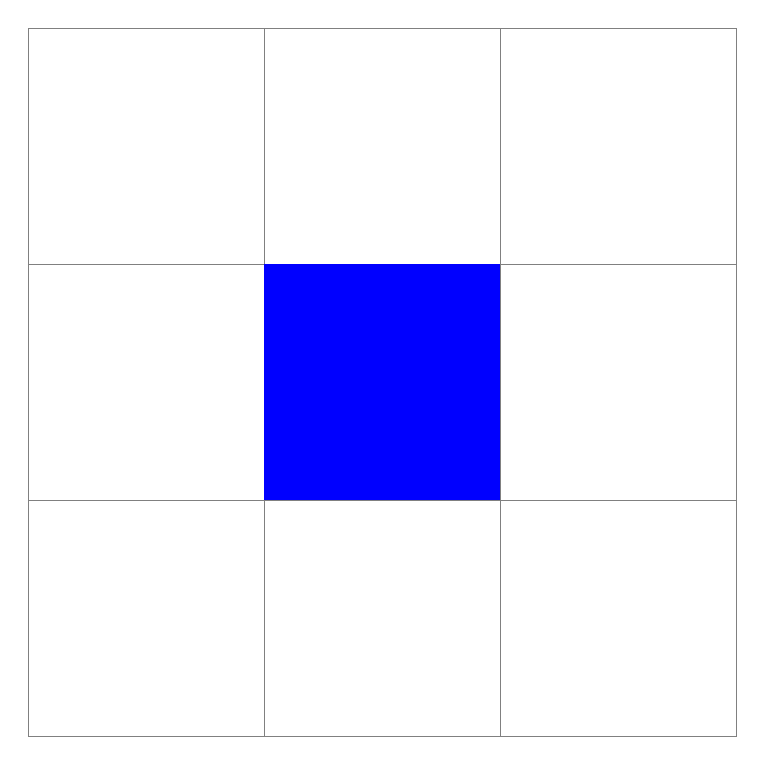
\begin{tikzpicture}
\draw[step=3cm,gray,very thin] (0,0) grid (9,9);
\fill[blue!] (6,6) rectangle (3,3);
\end{tikzpicture}
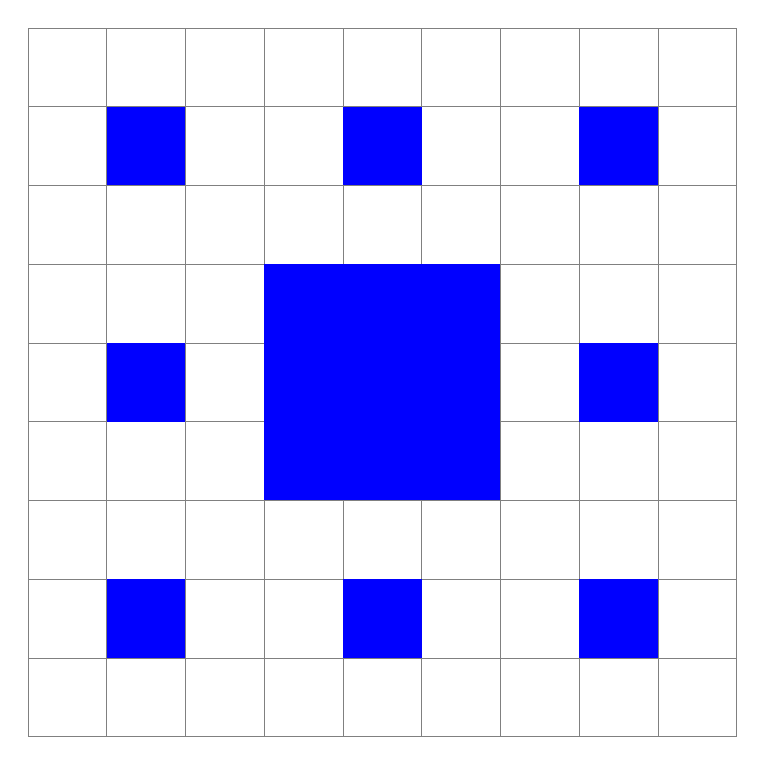
\begin{tikzpicture}
\draw[step=1cm,gray,very thin] (0,0) grid (9,9);
\fill[blue!] (6,6) rectangle (3,3);
\fill[blue!] (2,2) rectangle (1,1);
\fill[blue!] (5,2) rectangle (4,1);
\fill[blue!] (8,2) rectangle (7,1);
\fill[blue!] (2,8) rectangle (1,7);
\fill[blue!] (5,8) rectangle (4,7);
\fill[blue!] (8,8) rectangle (7,7);
\fill[blue!] (2,5) rectangle (1,4);
\fill[blue!] (8,5) rectangle (7,4);
\end{tikzpicture}
\section*{Problem B3}
\subsection*{(1)}
  Given that R is a regular language there exists a DFA
  $D = (Q, \Sigma, \delta, q_0, F)$ that accepts R i.e. $L(D) = R$.
  We will prove $L_1$ is regular by constructing
  an NFA $N$ using D that accepts $L_1$. Let $N = (Q \times 2^Q,
  \Sigma \cup \{\epsilon\}, \delta{'}, (q_0 , F), F')$ where the states in $N$
  are pairs consisting of a single state and a set of states. We define the
  transition function $\delta{'}$ as follows:
  \newline
  \indent $\forall a \in \Sigma$,\:$\delta{'}((p,S), a) = (\delta(p,a), S')$ where
  $S'= \{s'\,|\,\exists w \in \Sigma^*,\,|w| = 2,\, \delta^*(s',w) \in S\}$
  \newline
  \indent i.e. $S'$ is equal to the set of all states from which S is reachable
  via two transitions in D.
  \newline
  We can extend $\delta{'}$ to $\delta{'}^*$ as follows:
  \newline
  \indent $\forall u \in \Sigma^*\: \delta{'}^* ((p,S),u) = (\delta^* (p, u),S')$
  where $S' = \{s'\:|\:\exists v \in \Sigma^* ,\: |v|=2|u| ,\:
  \delta^* (s', v) \in S\}$
  \newline
  \indent i.e. $S'$ is equal to the set of all states from which S is reachable
  via $2|u|$ transitions in D.
  \newline
  Finally we define $F' = \{(p, S) \:|\: p \in S\}$ i.e. whenever the first element
  of the state is a member of the second element. Informally $N$ is an NFA which
  simulates traversing the DFA $D$ forwards and backwards simultaneously on any
  word $u \in \Sigma^*$ such that the transition function in $N$ makes one
  transition forward for each letter in $u$ starting from $q_0$ and two
  transitions backwards, starting from $F$, for every letter $a \in \Sigma$, thus
  accumulating a set of states that comprises the second part of a state in $N$.
  $N$ accepts a string $u$ when there exists a $v$ such that $uv \in R$ where
  $2|u| = |v|$ i.e. the state of the first element in an accepting state
  is a member of the set of states in the second element of an accepting state
  which means that $N$ ran forwards for some $u \in \Sigma^*$ and backwards for
  some $v \in \Sigma^*$ where $2|u| = |v|$ and ended in the same state.
  This by definition is the language $L_1$. Formal proof that $L(N) = L_1$ and
  thus that $L_1$ is a regular language:
  $$ L(N) = L_1 $$
  $$ \delta{'}^*((q_0, F), u) \in F' = \{u \:|\: \exists v \in \Sigma^* ,\:
  uv \in R ,\: |v| = 2|u|\}$$ 
  $$ \delta^*(q_0, u) \in \{q \:|\: \exists v \in \Sigma^* ,\:
  |v| = 2|u| ,\: \delta^*(q,v) \in F\}$$
  $$ \delta^*(q_0, u) = q ,\: \delta^*(q,v) \in F \implies$$
  $$\delta^*(q_0, uv) \in F \implies uv \in R ,\: |v| = 2|u|$$
  $$ u \in L(N) \implies u \in L_1$$

\subsection*{(2)}

\section*{Problem B4}
\subsection*{(a)}
  Let $D = (Q, \Sigma, q_0, \delta, F)$ be the DFA that accepts the regular
  language L, i.e. $L(D) = L$. We can construct a DFA for the language
  $Pre(L)$ as $D_{pre} = (Q, \Sigma, \delta, q_0, F')$ where we define
  $F' = \{q \:|\: \exists u,v \in \Sigma^* ,\: uv \in L
  ,\: \delta^* (q_0, u) = q ,\: \delta^* (q, v) \in F\}$.
  Informally, the accepting states in $D_{pre}$ are those states from which
  $F$ is reachable in $D$ via some reachable state $q \in Q$ and some
  word $v \in \Sigma^*$ i.e. it accepts all words $u \in \Sigma^*$
  such that such a $q$ and $v$ exist, or, the prefixes of L.
  Proof that $L(D_{pre}) = Pre(L)$ and thus that $Pre(L)$ is a regular language:
  $$u \in L(D_{pre}) \implies$$ $$\delta^*(q_0, u) \in F' =
  \delta^*(q_0, u) \in \{q \:|\: \exists v \in \Sigma* ,\: uv \in L
  ,\: \delta^*(q_0, u) = q\} \implies$$
  $$L(D_{pre}) = \{u \:|\: \exists v \in \Sigma^* ,\: uv \in L ,\:
  \exists q \in Q ,\: \delta^*(q_0, u) = q \}
  = Pre(L)$$
 
\subsection*{(b)}
  Let $D = (Q, \Sigma, q_0, \delta, F)$ be the DFA that accepts the regular
  language L, i.e. $L(D) = L$. We can construct an NFA for the language
  $Suf(L)$ as $N_{suf} = (Q\cup{q_1}, \Sigma, q_1, \delta{'}, F)$
  where $\delta{'}$ is defined as:
  $$\delta{'}(q, a) = \{\delta(q,a)\} \:|\: \forall q \in Q ,\: a \in \Sigma$$
  $$\delta{'}(q_1, \epsilon) = \{q \:|\: \exists u,v \in \Sigma^* ,\:
  uv \in L ,\: \delta^* (q,v) \in F ,\: \delta^* (q_0,u) = q\}$$
  which can be extended to $\delta{'}^*$ as follows:
  $$\delta{'}^*(q, v) = \{\delta^*(q,v)\} \:|\:
  \forall q \in Q ,\: v \in \Sigma^*$$
  $$\delta{'}^*(q_1, v) = \delta{'}^*(\delta{'}(q_1, \epsilon), v) =
  \{\delta^*(\delta{'}(q_1, \epsilon), v)\} \:|\: \forall v \in \Sigma^*$$
  Informally $N_{suf}$ starts at $q_1$ and makes
  an epsilon transition to any state $q$ from which there is a path to $F$ and
  there exists a path from $q_0$ to $q$ i.e. $N_{suf}$ excepts all words that
  are suffixes of words in $L$. Formally, here is a proof that
  $L(N_{suf}) = Suf(L)$ and thus that $Suf(L)$ is a regular language:
  $$ v \in L(N_{suf}) \implies \delta{'}^*(q_1, v) \in F =
  \delta^*(\delta{'}(q_1, \epsilon), v)$$
  \begin{center}where, by the following definiton:\end{center}
  $$\delta{'}(q_1, \epsilon) = \{q \:|\: \exists u,v \in \Sigma^* ,\:
  uv \in L ,\: \delta^* (q,v) \in F ,\: \delta^* (q_0,u) = q\}$$
  \begin{center}that\end{center}
  $$\delta^*(\delta{'}(q_1, \epsilon), v) = \delta^*(q, v)$$
  \begin{center}where\end{center}
  $$\delta^* (q,v) \in F ,\: \exists u \in \Sigma^* ,\: uv \in L ,\:
  \delta^* (q_0,u) = q$$
  $$ = Suf(L)$$

\subsection*{(c)}

\section*{Problem B5}
\subsection*{(a)} Prove that $L=L^+$ iff LL $\subseteq$ L.
\subsubsection*{Case $L=L^+ \implies LL \subseteq L$:}
$$L = L^+ = \bigcup\limits_{n\ge1} L^n$$
$$LL = L^2 \subseteq \bigcup\limits_{n\ge1} L^n$$
$$LL = L^2 \subseteq \bigcup\limits_{n\ge1} L^n = L$$

\subsubsection*{Case $LL \subseteq L \implies L^+ = L$:}
NOTES
\newline
Proof by induction on n where $L^+ = \bigcup\limits_{n\ge1} L^n$
Base Case: n = 1. So $L^n = L^1  = L$.
Inductive Case: Assume $L^n = L$.
Show $L^{n+1} =L$. 
\newline 
$L^{n+1} = LL^{n} = LL$. If we can show that $L \subseteq LL$, then 
$LL=L$.
STUCK. Use $(n \ge 1)$, $ \cup L^n$ to prove.
ENDNOTES

\subsection*{(b)}
($L=\emptyset$ or $L=L^*$) iff LL=L.
Recall $L^\ast = \bigcup\limits_{n \ge 0} L^n \implies L^n \subseteq L^\ast,
\forall n\ge 0$.
\newline
\subsubsection*{Case $\implies$:}
Prove ($L=\emptyset$ or $L=L^*$)
$\implies LL=L$. $L = L^\ast \implies {\epsilon } \in L$
Since ${\epsilon } \in L \implies L \subseteq LL = L^2 \implies L \subseteq LL$.
From part (a) we know $L=L^+ \implies LL \subseteq L$. 
$L \subseteq LL$ and $LL \subseteq L \implies L = LL$.

\subsubsection*{Case $\Longleftarrow$:} 
$L=LL \implies L = L^\ast$.
(The case where $L= \emptyset$ is trivial).
Claim: $L=L^2 \implies {\epsilon } \in L$ SHOW PROOF.
By part (a), $LL=L \implies LL \subseteq L \implies
L = L^+$ and since ${\epsilon } \in L$, $L^+=L^\ast$.

\section*{Problem B6}

\subsection*{(c)}
$ A1 = \le_1$ and $A2 = \le_2$ are wqo's.
The crossproduct ordering $(a_1,a_2) \le (b_1, b_2)
iff a_1 \le_1 b_1 and a_2 \le_2 b_2$.
Show $\le$ is also a wqo on $A_1 x A_2$.
Consider an infinite sequence $(s_i ' , s_i '') \in A_1 x A_2, i = 1,2,...$.
Have the prime sequence in A1 and have the double prime sequence in A2.
Use part (b), which says that if you have a wqo, that means the
(infinite sequence is "good") you can extend. Take first subsequence,
know it is in wqo (can extract a subsequence specified by the function f).
we knoe this subsequence is in incrasing order. use these indicies to extract
from infinite sequence.

\subsection*{(d)}
Prove the following result.
\newline
Let $n$ be any  integer such that $n>1$.
Given any infinite sequence $s_i$ with $i \ge 1$ of $n$-tuples of
natural numbers, there exist positive integers $i, j$ such that
$i<j$ and $s_{i}\preceq_{n} s_{j}$, where $\preceq_{n}$ is the
partial order on $n$-tuples of natural numbers
induced by the natural ordering $\le$ on $\mathbb{N}$
To prove: $A_i$'s are equal to $\mathbb{N}$.
So we can extend c by induction on $\preceq_{n}$ on $\mathbb{N}$.
Given that $\preceq_{n}$ is a preorder on A ($\preceq_{n} \subseteq AxA$),
then $\preceq_{n}$ is reflexive ($ x \preceq_{n} x,\forall x \in A$)
and transitive ($x \preceq_{n} y, y \preceq_{n} z \implies x \preceq_{n} z,
\forall x,y,z \in A$). NEED COMPLETE PROOF HERE.

\subsection*{(e)}
Let $\sqsubseteq$ be a preorder on a set $A$. We define the
preorder $\ll$ ({\it string embedding\/}) on $A^{*}$ as follows:
\newline
$\epsilon \ll u$ for each $u\in A^{*}$, and,
for any two strings $u=u_{1}u_{2}\ldots u_{m}$ and
$v=v_{1}u_{2}\ldots v_{n}$, $1\leq m\leq n$,
$$u_{1}u_{2}\ldots u_{m} \ll v_{1}v_{2}\ldots v_{n}$$
iff there exist  integers $j_{1},\ldots,j_{m}$ such that
$1\leq j_{1} < j_{2} < \ldots < j_{m-1} < j_{m} \leq n$ and
$$u_{1} \sqsubseteq v_{j_{1}},\ \ldots,\ u_{m} \sqsubseteq v_{j_{m}}.$$
\newline
Solution (part 1): Prove that $\ll$ is a preorder by showing (1) $u \ll u$ and
(2) $u \ll v, v \ll w \implies u \ll w$.
\newline
(1) By the definition of $\ll$, $u \ll u$ (with $u=u_{1}u_{2}\ldots u_{m}$) iff
there exist integers $j_{1},\ldots,j_{m}$ such that
$1\leq j_{1} < j_{2} < \ldots < j_{m-1} < j_{m} \leq m$ and
$u_{1} \sqsubseteq u_{j_{1}},\ \ldots,\ u_{m} \sqsubseteq u_{j_{m}}$.
This follows from definition of preorder $\sqsubseteq$ is reflexive.
\newline
(2) By the definition of $\ll$, $u \ll v$ (with $u=u_{1}u_{2}\ldots u_{m}$ and
$v=v_{1}v_{2}\ldots v_{n}$, $1\leq m\leq n$)
iff there exist integers $j_{1},\ldots,j_{m}$ such that
$1\leq j_{1} < j_{2} < \ldots < j_{m-1} < j_{m} \leq n$ and
$u_{1} \sqsubseteq v_{j_{1}},\ \ldots,\ u_{m} \sqsubseteq v_{j_{m}}.$
\newline
Additionally, by the definition of $\ll$, $v \ll w$
(with $v=v_{1}v_{2}\ldots v_{n}$ and $w=w_{1}w_{2}\ldots w_{p}$,
$1\leq n\leq p$) iff there exist integers $k_{1},\ldots,k_{n}$ such that
$1\leq k_{1} < k_{2} < \ldots < k_{n-1} < k_{n} \leq p$ and
$v_{1} \sqsubseteq w_{k_{1}},\ \ldots,\ v_{n} \sqsubseteq w_{k_{n}}$.
\newline
By the transitivity of preorder $\sqsubseteq
$, $u_{1} \sqsubseteq v_{j_{1}},\ \ldots,\ u_{m} \sqsubseteq v_{j_{m}}$
and $v_{1} \sqsubseteq w_{k_{1}},\ \ldots,\ v_{n} \sqsubseteq w_{k_{n}}
\implies u_{1} \sqsubseteq w_{k_{1}},\ \ldots,\ u_{n} \sqsubseteq w_{k_{n}}$.
And by the definition of $\ll$, $u_{1} \sqsubseteq w_{k_{1}},\ \ldots,\ u_{n}
\sqsubseteq w_{k_{n}} \implies u \ll w$.

\medskip

Solution (part 2): Prove that if $\sqsubseteq $ is a partial order,
$\ll$ is a partial order, by showing that $\ll$ is anti-symmetric.
If $\sqsubseteq $ is a partial order, then it must be anti-symmetric.
Let $u=u_{1}u_{2}\ldots u_{m}$ and $v=v_{1}v_{2}\ldots v_{n}$.
Show if u $\ll$ v, and v $\ll$ u, then u = v (definition of antisymmetry).
\newline
By the definition of $\ll$, $u \ll v$ (with $u=u_{1}u_{2}\ldots u_{m}$ and
$v=v_{1}v_{2}\ldots v_{n}$, $1\leq m\leq n$) iff there exist integers $j_{1},
\ldots,j_{m}$ such that $1\leq j_{1} < j_{2} < \ldots < j_{m-1} < j_{m} \leq n$
and $u_{1} \sqsubseteq v_{j_{1}},\ \ldots,\ u_{m} \sqsubseteq v_{j_{m}}$.
By the definition of $\ll$, $v \ll u$ (with $u=u_{1}u_{2}\ldots u_{m}$ and
$v=v_{1}v_{2}\ldots v_{n}$, $1\leq n\leq m$)
iff there exist integers $j_{1},\ldots,j_{n}$ such that
$1\leq j_{1} < j_{2} < \ldots < j_{n-1} < j_{n} \leq m$ and
$v_{1} \sqsubseteq u_{j_{1}},\ \ldots,\ v_{n} \sqsubseteq u_{j_{n}}.$
\newline
Because $\sqsubseteq $ is anti-symmetric, $u_{1} \sqsubseteq v_{j_{1}},\ \ldots,
\ u_{m} \sqsubseteq v_{j_{m}}$ and $v_{1} \sqsubseteq u_{j_{1}},\ \ldots,
\ v_{n} \sqsubseteq u_{j_{n}} \implies u = v.$

\medskip

Solution (part 3): Prove $\ll$ is the least preorder on $A^\ast$ satisfying:
\begin{enumerate}
\item[(1)] (deletion property)
$uv \ll uav$, for all $u, v\in A^{*}$ and $a\in A$;
\medskip
\item[(2)] (monotonicity) $uav \ll ubv$ whenever $a \sqsubseteq b$,
for all $u, v\in A^{*}$ and $a, b\in A$.
\end{enumerate}

\medskip

Must show $u \ll v \implies u \preceq v$ for any preorder $ \preceq $ that satisfies (1) and (2).
\newline
Show that $\forall n \ge 1, \forall u_i \in \Sigma^\ast , (1 \le i \le n+1)$ and $ \forall v_i \in \Sigma^\ast (1 \le i \le n)$,
$v_1...v_n \le u_1v_1u_2...u_nv_nu_{n+1}$. Prove by induction on length of $k= |u_1|+|u_2|+ ... +|u_{n+1}|.$ 
\newline
Base Case: k=0 is automatic. 
\newline
Inductive Case: There is some $u_i$ not equal to $ \epsilon$. Let $u_i = u_i ' a$, with $a \in A$.
\newline
Consider $u_1 ,u_2 , ... , u_i ' , ... , u_{n+1}$  so  $|u_1| + ... + |u_i '| + ... + |u_{n+1}| = k-1$. 
\newline
By the inductive hypothesis,
$v_1 ... v_n \le u_1 v_1 u_2 ... v_{i-1} u_i ' v_{i}...u_nv_nu_{n+1}$ by (1).

\medskip

Secondly, prove
$ \forall n \ge 1, \forall u_i \in \Sigma^\ast$ $(1 \le i \le n+1)$ and $\forall a_i,b_i \in \Sigma$ $(1 \le i \le n)$ 
if $a_i \sqsubseteq b_i, i \ge 1$.
\newline
$u_1a_1u_2...u_na_nu_{n+1} \le u_1b_1u_2...u_nb_nu_{n+1}$ by induction on n.
\newline
Base Case: $n=1$. This is exactly condition two. 
\newline 
Inductive Case: Apply the inductive hypothesis to the 
first n elements. Then set the first n elements to the value of u and apply (2) to get n + 1.
\medskip

Using these two facts for any strings u $\ll v \implies u \preceq v$ where $\preceq$ is a preorder satisfying (1) and 
(2) and $|u| \le |v|$. String embedding $u \ll v$ means if $u=a_1 ...a_n$, then $v=w_1 b_1 ... b_n w_{n+1}$
with $a_i \sqsubseteq b_i$ and $w_i \epsilon A^{\ast}$. So, $a_1 ... a_n  \preceq w_1 a_1 w_2 ... w_n a_n w_{n+1}$, then convert
a's to b's with proven part 2. $a_1 ... a_n  \preceq w_1 a_1 w_2 ... w_n a_n w_{n+1} \preceq w_1 b_1 w_2 ... w_n b_n w_{n+1}$.

\end{document}
